\documentclass[main.tex]{subfiles}
\begin{document}

Các bạn có thể copy nội dung của các đoạn code trong phần này trong thư mục \code{answer-sources} ở link sau: \href{https://github.com/hungngocphat01/nes-ktlt-2021}{Github: hungngocphat01/nes-ktlt-2021}.
%%%%%%%%%%%%%%%%%%%%%%%%%%%%%%%%%%%%%%%%%%%%%
\subsection{Con trỏ cơ bản}
\textit{Lưu ý: các địa chỉ của các ô nhớ trong những hình dưới đây chỉ mang tính chất minh hoạ}.

\subsubsection{Câu a}
Do \code{p} là một con trỏ, trỏ đến \code{a} nên \code{*p} chính là \code{a}. Phép gán \code{*p += 4} tương đương \code{a += 4} nên đáp án là \code{19.75}.

\subsubsection{Câu b}
Do \code{p} trỏ đến cùng vùng nhớ với \code{a}, nên các thao tác truy xuất bộ nhớ thông qua \code{p} cũng hoàn toàn tương tự với các thao tác truy xuất bộ nhớ thông qua \code{a}.

\begin{center}
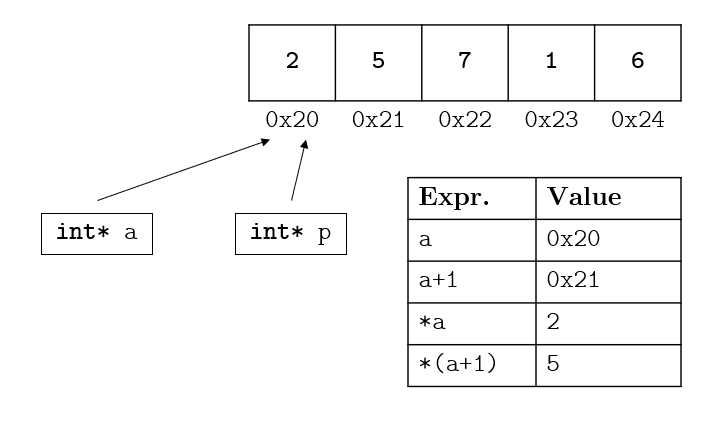
\includegraphics[width=0.7\textwidth]{image/ans_CTRLCB_b.png}
\end{center}

Ta thấy \code{*(p+1)} trùng với \code{*(a+1)}, chính là \code{a[1]}. Còn \code{*a} chính là \code{a[0]}, có giá trị là \code{2}.\\
Vậy \code{*(p + 1) += *a;} tương đương với phép gán \code{a[1] += a[0]}.\\
Tương tự, \code{cout << *(a + 1);} là \code{cout << a[1]}, nên kết quả in ra màn hình sẽ là \code{7}.

\subsubsection{Câu c}
\begin{figure}[H]
\centering
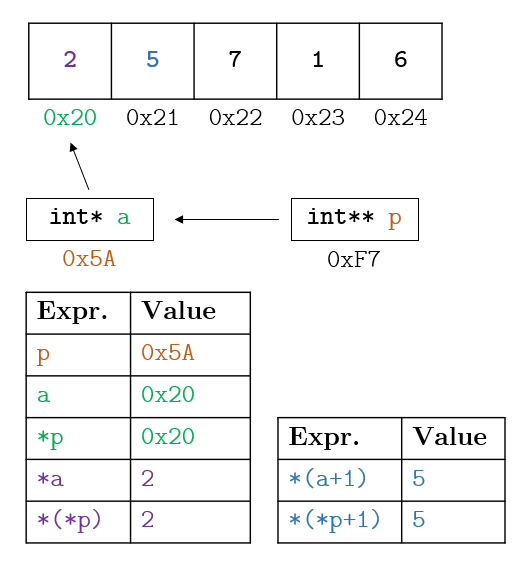
\includegraphics[width=0.5\textwidth]{image/ans_CTRLCB_c.png}
\end{figure}

Do \code{p} là một con trỏ, trỏ đến \code{a} nên \code{*p} chính là \code{a}. \\
\code{(*p)[4]} tương đương với \code{a[4]}, \code{*(*p + 1)} tương đương với \code{*(a + 1)}, chính là \code{a[1]}. Tự suy luận, ta có kết quả là \code{7}.

\subsubsection{Câu d}
Ta thấy \code{*(a+2)} chính là \code{a[2]}. \\
Nếu ta đặt \code{u = *(a+2)} thì \code{(*(a+2)+1)} sẽ trở thành \code{*(u+1)}, chính là \code{u[1]}.\\
Mà vì \code{u = *(a+2) = a[2]} nên \code{u[1]} chính là \code{a[2][1]}.\\
Giá trị tại vị trí \code{a[2][1]} chính là \code{5}.

Trên đây là một cách giải thích theo phong cách ``toán học''. Nếu các bạn muốn một cách giải thích theo bản chất của con trỏ có thể tham khảo hình dưới đây (tự tham khảo):
\begin{figure*}
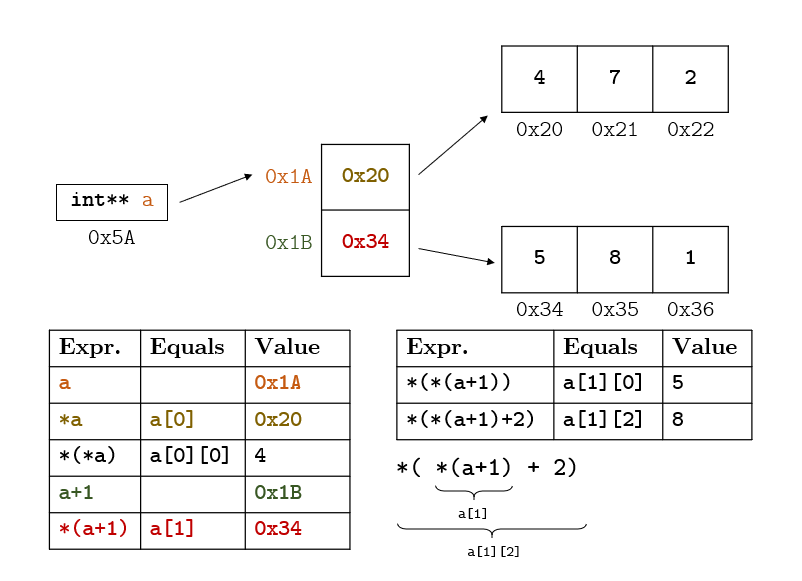
\includegraphics[width=0.6\textwidth]{image/ans_CTRLCB_d.png}
\end{figure*}

%%%%%%%%%%%%%%%%%%%%%%%%%%%%%%%%%%%%%%%%%%%%%

\subsection{Con trỏ nâng cao}
\subsubsection{Câu a}
\inputminted[linenos]{cpp}{answer_sources/ConTroNC_a.cpp}

\subsubsection{Câu b}
Nhắc lại kiến thức về con trỏ 2 cấp:\\
\begin{figure*}
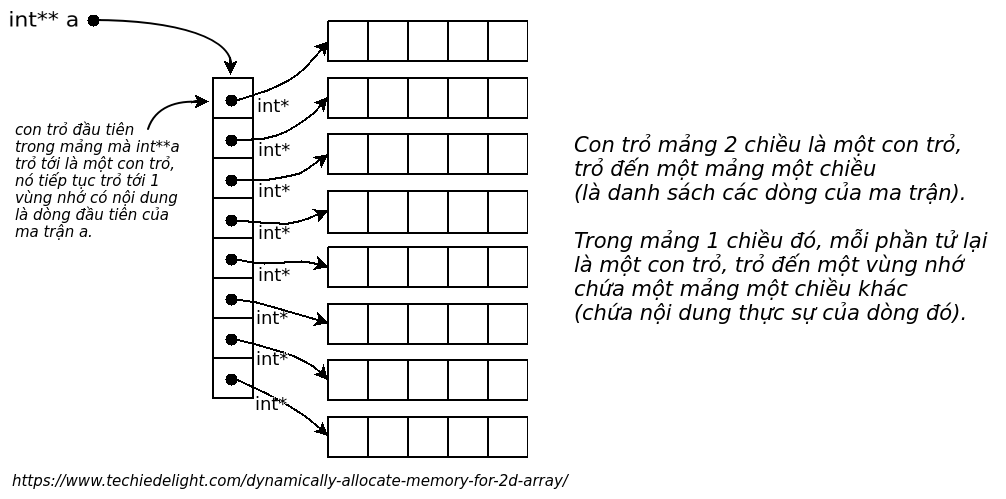
\includegraphics[width=1\textwidth]{image/ans_CTRLNC_1.png}
\end{figure*}

\inputminted[linenos]{cpp}{answer_sources/ConTroNC_b.cpp}
\textit{Lưu ý: Ta phải giải phóng các phần tử của a trước khi giải phóng a, vì bản thân a chỉ là một con trỏ 2 cấp, nó không thực sự chứa nội dung của ma trận. Khi ta giải phóng a thì các con trỏ thành phần bên trong a vẫn còn tồn tại, gây rò rỉ bộ nhớ nếu như ta không giải phóng trước.}

\begin{center}
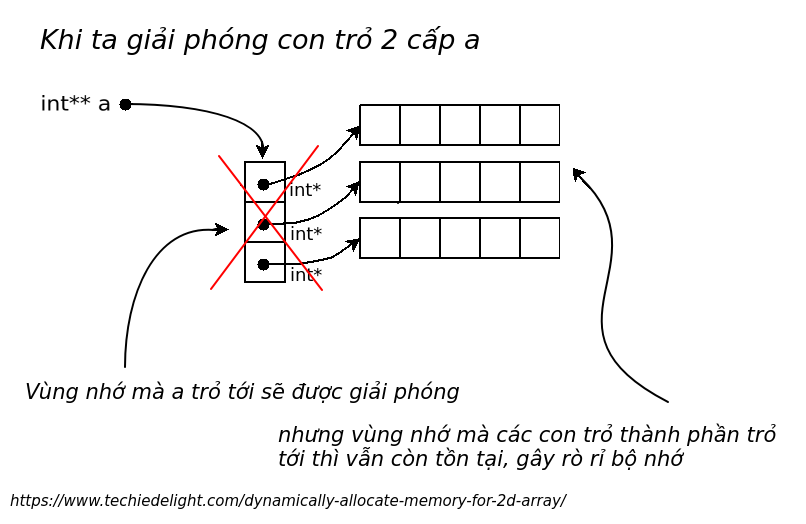
\includegraphics[width=0.8\textwidth]{image/ans_CTRLNC_2.png}
\end{center}


\subsubsection{Câu c}
\inputminted[linenos]{cpp}{answer_sources/ConTroNC_c.cpp}

%%%%%%%%%%%%%%%%%%%%%%%%%%%%%%%%%%%%%%%%%%%%%

\subsection{Danh sách liên kết}
\inputminted[linenos]{cpp}{answer_sources/DanhSachLK.cpp}

%%%%%%%%%%%%%%%%%%%%%%%%%%%%%%%%%%%%%%%%%%%%%

\subsection{Ngăn xếp, hàng đợi}
\subsubsection{Ngăn xếp}
Ta để ý là các cặp dấu ngoặc xuất hiện theo thứ tự 
first in first out, có nghĩa là dấu mở ngoặc nào tới sau thì nó phải được đóng trước. Do đó ta sử dụng stack để giải bài toán này. Cụ thể như sau:
\begin{itemize}
    \item Ta duyệt qua từng kí tự của chuỗi đó.
    \item Nếu ta gặp một dấu mở ngoặc, ta đẩy nó vào stack.
    \item Nếu ta gặp một dấu đóng ngoặc, ta kiểm tra thử nó có cùng loại với dấu mở ngoặc mà ta gặp gần nhất hay không (dấu mở ngoặc gần nhất là phần tử trên đỉnh stack). Nếu có, ta tiếp tục xét kí tự tiếp theo. Nếu khác loại thì coi như chuỗi là không hợp lệ (trường hợp này là bị thiếu dấu mở ngoặc, dư dấu đóng ngoặc).
    \item Sau khi duyệt hết các kí tự trong chuỗi, ta kiểm tra xem trong stack còn dư phần tử nào hay không, nếu có thì ta đã rơi vào trường hợp dư dấu mở ngoặc, thiếu dấu đóng ngoặc.
    \item Nếu chuỗi nhập vào không vi phạm bất cứ tiêu chuẩn nào thì nó là hợp lệ.
\end{itemize}

\inputminted[linenos]{cpp}{answer_sources/Stack.cpp}

%%%%%%%%%%%%%%%%%%%%%%%%%%%%%%%%%%%%%%%%%%%%%

%%%%%%%%%%%%%%%%%%%%%%%%%%%%%%%%%%%%%%%%%%%%%

\subsection{Đệ quy}
Nhắc lại về thuật toán Selection Sort:
\begin{itemize}
	\item Chọn ra phần tử nhỏ nhất trong n phần tử ban đầu.
	\item Hoán đổi phần tử đó lên đầu mảng.
	\item Bỏ qua phần tử đầu tiên, ta xem phần tử tiếp theo như là đầu mảng và tiếp tục lặp lại thuật toán cho đến khi hết mảng.
\end{itemize}

Ta có thể cài đặt một thuật toán đệ quy trên DSLK như sau:

\begin{minted}{cpp}
void recursiveSelectionSort(Node* head);
\end{minted}

\begin{itemize}
	\item Tìm phần tử nhỏ nhất trong danh sách liên kết.
	\item Hoán đổi node nhỏ nhất đó lên đầu dãy.
	\item Gọi hàm sắp xếp đệ quy cho dãy có \code{head} là \code{head->next}.
\end{itemize}

\inputminted[linenos]{cpp}{answer_sources/DeQuy.cpp}

\subsection{Quy hoạch động}
Vì quy hoạch động ở mức độ nhập môn chỉ là một bài toán đệ quy đã được tối ưu, nên các bạn phải có ý tưởng để giải bài toán đó bằng đệ quy thông thường trước. Nhìn chung, khi giải một bài toán có sử dụng quy hoạch động, ta cần làm 2 bước sau:
\begin{itemize}
	\item Đưa ra ý tưởng giải bài toán bằng phương pháp vét cạn (đệ quy thông thuờng) trước:
		\begin{itemize}
			\item Thử làm bài toán đó bằng tay và rút ra thuật toán thực hiện.
			\item Mô hình hoá thứ tự các bước thực hiện dưới dạng đồ thị.
			\item Trình bày thuật toán bằng đệ quy.
		\end{itemize}
	\item Tối ưu hoá:
		\begin{itemize}
			\item Thêm một ``bảng ghi nhớ'' vào hàm đệ quy đã viết ở bước trước.
			\item Mỗi khi gọi hàm, tra bảng và trả về giá trị đã được lưu, nếu không có thì bắt đầu thực thi quá trình tính toán và lưu giá trị vào bảng ghi nhớ đó.
		\end{itemize}
\end{itemize}

Bạn có thể tham khảo thêm trong khoá học dài 5 tiếng về quy hoạch động của \code{freeCodeCamp} (tiếng Anh): \href{https://www.youtube.com/watch?v=oBt53YbR9Kk}{Youtube: Dynamic Programming - Learn to Solve Algorithmic Problems \& Coding Challenges}. Bài toán trên nằm ở \code{1:52:07}.

\subsubsection{Phân tích bài toán}
Ta có thể đưa bài toán trên về một dạng tổng quát hơn:\\
Cho mảng nguyên dương \code a và một số nguyên dương \code{n}. Hãy tìm ra một giỏ được lấy từ các phần tử trong \code a (giỏ giống như tập hợp nhưng các phần tử có thể lặp lại được), sao cho tổng các phần tử của giỏ đó có giá trị bằng \code{n} và cho số lượng phần tử trong giỏ đó là nhỏ nhất?

\textbf{Giả sử ta có \code{a = \{7, 3, 6, 2\}} và \code{n = 8}}. Để biết được các phần tử nào cộng lại có giá trị là 8, ta làm theo các bước sau:
\begin{itemize}
    \item Giả sử ta có một dãy các phần tử  $a = {a_1, a_2, a_3, ..., a_m}$.
    \item Nếu $a_i+a_j+a_k+...=n$ ($0 \le i \le j \le k \le ... < m $) thì ta có $n-a_i-a_j-a_k-...=0$.\par
    $\Rightarrow$ Phương pháp để biết được liệu $n$ có thể phân tích thành các phần tử trong $a$ hay không là đem $n$ lần lượt trừ đi các phần tử trong $a$. Nếu $n$ trừ cho dãy các phần tử nào trong $a$ mà ra $0$ thì ta biết được dãy đó có tổng bằng chính $n$.
\end{itemize}

\subsubsection{Mô phỏng thuật toán bằng đồ thị}
Giả sử ta có \code{a = \{7, 3, 6, 2\}} và \code{n = 8}.
Ta lần lượt lấy \code{n = 8} trừ cho các phần tử trong \code{a}.

\begin{center}
\begin{forest}
for tree = {
    circle, draw,
    s sep+ = 10mm,
    l sep+ = 6mm,
    EL/.style = {
        edge label={node[midway, fill=white, inner sep=2pt, anchor=center]{#1}},
    },
    LV/.style = {
        draw=blue
    }
}
    [8,LV
        [1,EL=7]
        [5,EL=3]
        [2,EL=6]
        [6,EL=2]
    ]
\end{forest}
\par Quy ước kí hiệu: số 7 trên đường nối giữa 8 và 1 nghĩa là lấy 8-7=1
\end{center}

Ứng với mỗi hiệu thu được, ta tiếp tục thực hiện đệ quy, lại lấy nó lần lượt  trừ cho các phần tử trong \code a. Dưới đây là ví dụ cho node số 6.

\begin{center}
    \begin{forest}
    for tree = {
        circle, draw,
        s sep+ = 10mm,
        l sep+ = 6mm,
        EL/.style = {
            edge label={node[midway, fill=white, inner sep=2pt, anchor=center]{#1}},
        },
        LV/.style = {
            draw=blue
        }
    }
    [8
        [1,EL=7]
        [5,EL=3]
        [2,EL=6]
        [6,EL=2,LV
            [-1,EL=7]
            [3,EL=3]
            [0,EL=6]
            [4,EL=2]
        ]
    ]
\end{forest}
\end{center}

Ta tiếp tục thực hiện cho các node \code{1, 5, 2}  còn lại. Để tiết kiệm không gian, tụi mình sẽ không ghi các node có giá trị âm.

\begin{center}
    \begin{forest}
    for tree = {
        circle, draw,
        s sep+ = 10mm,
        l sep+ = 6mm,
        EL/.style = {
            edge label={node[midway, fill=white, inner sep=2pt, anchor=center]{#1}},
        },
        LV/.style = {
            draw=blue
        }
    }
    [8
        [1,EL=7,LV]
        [5,EL=3,LV
            [2,EL=3]
            [3,EL=2]
        ]
        [2,EL=6,LV
            [0,EL=2]
        ]
        [6,EL=2,LV
            [0,EL=6]
            [3,EL=3]
            [4,EL=2]
        ]
    ]
\end{forest}
\end{center}
Với những hiệu thu được, ta lại tiếp tục đệ quy, lại lấy chúng trừ cho các phần tử trong \code{a}. Nếu hiệu âm, chúng ta sẽ bỏ qua (tụi mình sẽ không vẽ lại).

\textit{Cụ thể: Ở số 1, do nó không thể trừ cho bất cứ phần tử nào trong \code a được nữa (vì nếu trừ hiệu của chúng sẽ âm) nên tụi mình không vẽ lại.}

\begin{center}
    \begin{forest}
    for tree = {
        circle, draw,
        s sep+ = 10mm,
        l sep+ = 6mm,
        EL/.style = {
            edge label={node[midway, fill=white, inner sep=2pt, anchor=center]{#1}},
        },
        MK/.style = {
            edge = red
        },
        LV/.style = {
            draw=blue
        },
    }
    [8
        [1,EL=7]
        [5,EL=3
            [2,EL=3,LV
                [0,EL=2]
            ]
            [3,EL=2,LV
                [0,EL=3]
                [1,EL=2]
            ]
        ]
        [2,EL=6
            [0,EL=2]
        ]
        [6,EL=2
            [0,EL=6]
            [3,EL=3,LV
                [0,EL=3]
                [1,EL=2]
            ]
            [4,EL=2,LV
                [1,EL=3]
                [2,EL=2]
            ]
        ]
    ]
\end{forest}
\end{center}

Ta tiếp tục thực hiện đệ quy với bậc cuối cùng 
\begin{center}
    \begin{forest}
    for tree = {
        circle, draw,
        s sep+ = 10mm,
        l sep+ = 6mm,
        EL/.style = {
            edge label={node[midway, fill=white, inner sep=2pt, anchor=center]{#1}},
        },
        MK/.style = {
            edge = red
        },
        LV/.style = {
            draw=blue
        },
    }
    [8
        [1,EL=7]
        [5,EL=3
            [2,EL=3
                [0,EL=2]
            ]
            [3,EL=2
                [0,EL=3]
                [1,EL=2]
            ]
        ]
        [2,EL=6
            [0,EL=2]
        ]
        [6,EL=2
            [0,EL=6]
            [3,EL=3
                [0,EL=3]
                [1,EL=2]
            ]
            [4,EL=2
                [1,EL=3]
                [2,EL=2,LV
                    [0,EL=2]
                ]
            ]
        ]
    ]
\end{forest}
\end{center}

Hoàn thành giải thuật đệ quy, ta thu được đồ thị sau:
\begin{center}
    \begin{forest}
    for tree = {
        circle, draw,
        s sep+ = 10mm,
        l sep+ = 6mm,
        EL/.style = {
            edge label={node[midway, fill=white, inner sep=2pt, anchor=center]{#1}},
        },
        MK/.style = {
            edge = red
        },
        LV/.style = {
            draw=blue
        },
    }
    [8
        [1,EL=7]
        [5,EL=3,MK
            [2,EL=3,MK
                [0,EL=2,MK]
            ]
            [3,EL=2,MK
                [0,EL=3,MK]
                [1,EL=2]
            ]
        ]
        [2,EL=6,MK
            [0,EL=2,MK]
        ]
        [6,EL=2,MK
            [0,EL=6,MK]
            [3,EL=3,MK
                [0,EL=3,MK]
                [1,EL=2]
            ]
            [4,EL=2,MK
                [1,EL=3]
                [2,EL=2,MK
                    [0,EL=2,MK]
                ]
            ]
        ]
    ]
\end{forest}
\end{center}
Quan sát đồ thị trên, ta có thể dễ dàng thấy được các bộ số sau là những bộ số cần tìm. Chúng đều có tổng bằng 8.
\begin{itemize}
    \item 3, 3, 2
    \item 3, 2, 3
    \item \textbf{6, 2}
    \item \textbf{2, 6}
    \item 2, 3, 3
    \item 2, 2, 2, 2
\end{itemize}

Bỏ qua các dãy trùng nhau, ta dễ dàng thấy được \code{2, 6} chính là dãy có số phần tử nhỏ nhất.

\subsubsection{Tối ưu hoá bài toán bằng bảng tra lời giải}
Xét lại mô hình ở trên ta đã mô tả, có thể dễ dàng thấy được các node được tô màu bị giải đi giải lại nhiều lần, rất là mất thời gian nếu số lượng node lớn. Do đó ta nên sử dụng quy hoạch động (bảng tra lời giải) để giải. 

\begin{center}
    \begin{forest}
    for tree = {
        circle, draw,
        s sep+ = 10mm,
        l sep+ = 6mm,
        EL/.style = {
            edge label={node[midway, fill=white, inner sep=2pt, anchor=center]{#1}},
        },
        BLC/.style = {
            draw=blue
        },
        RDC/.style = {
            draw=red
        },
    }
    [8
        [1,EL=7]
        [5,EL=3
            [2,EL=3,BLC
                [0,EL=2]
            ]
            [3,EL=3,RDC
                [0,EL=3]
                [1,EL=2]
            ]
        ]
        [2,EL=6,BLC
            [0,EL=2]
        ]
        [6,EL=2
            [0,EL=6]
            [3,EL=3,RDC
                [0,EL=3]
                [1,EL=2]
            ]
            [4,EL=2
                [1,EL=3]
                [2,EL=2,BLC
                    [0,EL=2]
                ]
            ]
        ]
    ]
\end{forest}
\end{center}

Giả sử cho \code{a = \{1, 2, 5, 25 \}} và \code{n = 100}. Nhìn bằng mắt thường, ta có thể thấy ngay dãy ngắn nhất là \code{25 + 25 + 25 + 25}, nhưng với giải thuật ở trên, nó sẽ chạy rất lâu nếu không dùng quy hoạch động. Máy mình xài \code{AMD Ryzen 5 PRO 4650U} mà nó giải 12 phút rồi vẫn chưa ra. Sau khi áp dụng quy hoạch động, đáp án được giải ra dưới 1 giây.
\footnote{\scriptsize Chip AMD kia văn phòng nhưng mà các bạn đừng nghĩ nó yếu nên giải lâu. Hiệu năng nó ăn đứt mấy con i5 gaming đời 9-10 dù TDP chỉ bằing 1/2 và có 1 quạt. Đã thử cả stress test (benchmark) và software rendering (thực tế), đến tụi mình cũng bất ngờ :)}

Chúng ta áp dụng quy hoạch động vào giải thuật đệ quy theo các bước sau:
\begin{itemize}
    \item Thêm một biến mảng vào tham số của hàm. Mảng này sẽ chứa các \textit{lời giải cho các bài toán con} (phương pháp này gọi là \code{memoization} hoặc là \code {cache}). Mỗi phần tử của mảng này là một mảng lưu số đồng xu mỗi loại.
    \item Trước khi thực hiện giải bài toán, ta sẽ kiểm tra xem trong \code{cache} đã chứa lời giải cho bài toán con này chưa? Nếu có, trả về kết quả. Nếu chưa, tiếp tục thực hiện giải thuật đệ quy như bình thường.
    \item Sau khi thực hiện xong giải thuật đệ quy, ta tiến hành lưu đáp án vừa giải vào mảng \code{cache} để sử dụng cho lần sau.
\end{itemize}
Vậy muốn đưa một giải thuật đệ quy thông thường về quy hoạch động, ta chỉ cần thêm 2 đoạn code là kiểm tra lời giải đã có chưa, và lưu lời giải vào mảng \code cache nếu đã giải xong.
\textit{Lưu ý: memoization chỉ là một phương pháp để giải quy hoạch động. Có rất nhiều hướng tiếp cận khác nhau cho quy hoạch động và sẽ có những bài toán mà memoization không thể thực hiện được}.


Dưới đây là bài toán trên được cài đặt theo quy hoạch động:
\inputminted[linenos,breaklines]{cpp}{answer_sources/QuyHoachDong_ToiUu.cpp}

{\scriptsize Tụi mình khuyên các bạn nên xài Python hay Javascipt để học thuật toán vì khi đó bạn sẽ chú tâm đến việc cài đặt thuật toán hơn là cài đặt mấy thứ linh tinh như cấp phát động hay kiểm soát vùng nhớ. Ngay cả khi có xài vector, việc cài đặt bài toán này trong C++ cũng sẽ rất khó khăn}.


%%%%%%%%%%%%%%%%%%%%%%%%%%%%%%%%%%%%%%%%%%%%%

\subsection{Bài tập tự luyện ở nhà}
Lưu ý: trong file pdf, phần giải thích này chỉ có giải thích, không có code. Các bạn vui lòng vào link được đính kèm ở đầu section để xem code.
\subsubsection{Cấp phát động}
Không có gì phải giải thích nhiều, thực hiện tương tự như khi thao tác với ma trận số nguyên.
Cần lưu ý khi truyền một con trỏ trỏ đến kiểu dữ liệu \code{T} vào hàm, mà ta muốn thay đổi giá trị của con trỏ đó (như cấp phát hay xoá) thì ta cần phải truyền dưới dạng tham chiếu: 
\begin{minted}{cpp}
void foo(T* &ptr) {
    ptr = new T[n];
    delete[] ptr;
}
\end{minted}
Hoặc dưới dạng tham trỏ
\begin{minted}{cpp}
void foo(T** ptr) {
    *ptr = new T[n];
    delete[] *ptr;
}
\end{minted}

%--------------------------------------------%
\subsubsection{Ngăn xếp}
\textbf{Nhắc lại về 2 cấu trúc:}
\begin{itemize}
    \item Stack: phần tử nào vào sau thì ra trước (như một chồng dĩa).
    \item Queue: phần tử nào vào sau thì ra sau (như một hàng người đợi mua trà sữa).
\end{itemize}

\textbf{Để implement một queue bằng 2 stack, ta có thể làm như sau}:
\begin{itemize}
    \item Giả sử ta có 2 stack gọi là stack (1) và stack (2).
    \item Khi push một phần tử vào queue, ta push vào (1).
    \item Khi muốn xem một phần tử ở đầu queue, vì phần tử ở đầu queue lại nằm dưới đáy của stack (1), nên ta pop tất cả phần tử từ stack (1) và chuyển qua stack (2). Lúc này, phần tử ở đầu queue đã nằm trên đỉnh của stack (2). Sau khi xem xong thì ta lại pop tất cả phần tử từ stack (2) bỏ về stack (1).
    \item Khi muốn xóa một phần tử khỏi queue, ta cũng chuyển tất cả phần tử từ (1) sang (2), nhưng sau đó phải bỏ phần tử trên đỉnh của stack (2) đi, rồi mới chuyển về lại stack (1).
\end{itemize}

\textbf{Ảnh động minh hoạ:}
\begin{itemize}
    \item Link ảnh GIF xem đỉnh queue: \href{https://ibb.co/64Hv1bH}{https://ibb.co/64Hv1bH}
    \item Link ảnh GIF xóa đỉnh queue: \href{https://ibb.co/syPCBFS}{https://ibb.co/syPCBFS}
\end{itemize}

\textbf{ Tối ưu hóa:}
Vì mỗi lần xem đỉnh queue ta phải pop (1) bỏ sang (2) rồi lại phải bỏ về (1), do đó ta nên tạo một biến tên là \code{top} bên trong struct queue của chúng ta để lưu giá trị của đỉnh queue để truy xuất thuận tiện hơn. Biến này sẽ được cập nhật giá trị khi và chỉ khi:
\begin{itemize}
    \item Khi queue đang rỗng mà chúng ta thêm một phần tử mới vào, thì phần tử đó sẽ là đỉnh của queue (các phần tử khác sau đó nằm ở phía sau phần tử đầu).
    \item Khi ta pop đỉnh của queue mà trong queue vẫn còn dữ liệu thì đỉnh queue sẽ là phần tử ngay kế sau.
\end{itemize}
%--------------------------------------------%


\end{document}
